\chapter{Asking a Billionaire Lawyer How to Make \$1,000,000}

This chapter reads the School of Hard Knocks interview with John Morgan as a case study in professional-service wealth. The source is not a blackboard lecture with visible equations; the useful mathematics is business arithmetic: bounded versus outcome-linked revenue, founder bottlenecks, distribution, advertising spend, trial capacity, debt, and trust. The claims are treated as transcript-backed interview claims, curated by LazyingArt LLC through Video2Book, not as independently audited financial statements.

\section{A Rare Route to Billionaire Status}

The opening move is not subtle, and it should not be made subtle in the notes. The host tells us that he is about to interview a billionaire in Florida, then names John Morgan and frames the unusual feature of the story: the fortune is said to have come through personal injury law. This matters because law, unlike software or finance, is usually imagined as a high-income profession rather than a scalable billionaire machine.

The first numerical facts are therefore status claims and scale claims:

\begin{align}
N_{\mathrm{Forbes}} &\approx \$1.5\mathrm{B},\\
F_{\mathrm{annual\ fees}} &\approx \$2\mathrm{B},\\
D_{\mathrm{debt}} &= 0.
\end{align}

Here \(N_{\mathrm{Forbes}}\) is the host's Forbes-attributed net-worth figure, \(F_{\mathrm{annual\ fees}}\) is Morgan's later statement that the firm did about \$2 billion in fees, and \(D_{\mathrm{debt}}\) records his repeated statement that he has no debt. We keep these quantities as interview evidence. They set the puzzle; they do not settle it.

A small law practice can be lucrative while remaining trapped inside the working life of one lawyer. Morgan's first answer to the scaling question is therefore important: the decisive move was not a legal theory, but delegation, trusted partners, and sharing the economics.

\section{Scale Begins With Partners, Not Employees}

Morgan says the way to scale is to delegate, get partners one can trust, and share the business with them. The language is plain: great people must make money with you, not just for you. That turns a law practice from a single professional's workload into an organization.

The founder-only constraint can be written as

\begin{equation}
\mathrm{Output}_{\mathrm{solo}}
\leq
\mathrm{capacity}_{\mathrm{founder}}.
\end{equation}

That inequality is the bottleneck. The partner model changes the object being built:

\begin{equation}
\mathrm{Output}_{\mathrm{firm}}
\approx
\sum_{i=1}^{n} q_i c_i,
\end{equation}

where \(c_i\) is the operating capacity of partner \(i\), and \(q_i\) is a rough trust-and-quality factor. This is a reconstruction, not Morgan's notation. It captures the mechanism: adding people only scales the firm when they add dependable capacity rather than supervision burden.

\subsection{Question \& Answer}

\paragraph{Question.}
How does a law practice stop being one person's job and become a multibillion-dollar firm?

\paragraph{Answer.}
It must stop requiring the founder's attention at every important point. Morgan's practical test is the ``send-delete'' person: someone who can receive a task, handle it, and let the sender delete the worry. In these notes, the operating value of such a person is

\begin{equation}
\mathrm{Attention\ returned}
=
\mathrm{Task\ delegated}
-
\mathrm{Followup\ required}.
\end{equation}

The lower the followup required, the more the operator expands the firm. Trust is therefore not a soft virtue in this model. It is a capacity multiplier.

\section{Pain, Purpose, and the First Work Ethic}

The interview then backs up from scale to motive. Morgan says his brother Tim was paralyzed at C6--C7 when Morgan was in college, and that the way Tim was treated changed his life. He says that when he sees clients, he sees Tim, and wants to treat them as Tim should have been treated.

That sequence should remain concrete:

\begin{enumerate}
\item A family injury creates anger at how an injured person is treated.
\item The anger gives law school a clear target.
\item The practice becomes a repeated promise to protect clients.
\end{enumerate}

The chapter should not turn this into generic uplift. The transcript presents personal injury law as a market, but also as an emotional category Morgan already understood before he built the business.

The host then asks whether Morgan came from money. Morgan says no, and moves quickly to early work: paper routes, selling cards at seven years old, and the belief that entrepreneurial drive shows itself early. A paper route matters in his telling because it is daily, repetitive, and unforgiving:

\begin{equation}
\mathrm{Early\ hustle}
\sim
\mathrm{daily\ obligation}
+
\mathrm{customer\ responsibility}
+
\mathrm{no\ vacation}.
\end{equation}

This is not a biological law. It is Morgan's claim, reconstructed as a note: repeated responsibility is the evidence he looks for when he talks about entrepreneurial temperament.

\section{Upside, Contingency Fees, and Negotiation Silence}

The next turn is business-model arithmetic. Asked what advice he would give a law student, Morgan contrasts hourly billing with his own contingency-fee model. The transcript is imperfect here, but the meaning is clear enough: he does not want to charge by the hour because there is not enough upside. He gets paid if he wins.

A cautious reconstruction is

\begin{align}
R_{\mathrm{hourly}} &= r h,\\
R_{\mathrm{contingency}} &=
\begin{cases}
0, & \mathrm{if\ the\ case\ loses},\\
\alpha S, & \mathrm{if\ the\ case\ wins},
\end{cases}
\end{align}

where \(r\) is an hourly rate, \(h\) is billable time, \(S\) is settlement or verdict value, and \(\alpha\) is an unspecified contingency share. The transcript does not give \(\alpha\), so the notes should not invent a percentage.

\subsection{Question \& Answer}

\paragraph{Question.}
Why reject hourly billing if hourly billing is more predictable?

\paragraph{Answer.}
Because predictability can cap the result. In the hourly model, revenue scales linearly with time. In the contingency model, the firm accepts downside risk in exchange for participation in the outcome. Morgan's claim is not that every lawyer should prefer contingency work. His narrower point is that the empire he wanted required upside tied to winning, not merely hours worked.

The interview then turns to negotiation. Morgan gives the familiar rule that whoever speaks first loses, but he immediately gives the mechanism: listening. People who talk too much do not hear. The negotiator first sizes up the deal and the person, then decides.

\begin{equation}
\mathrm{Move}_{t+1}
=
f(\mathrm{information\ heard}_{t},\ \mathrm{person}_{t},\ \mathrm{deal}_{t}).
\end{equation}

Speaking too early reduces the information set. In this part of the interview, silence is not passivity; it is data collection.

\section{Reputation, Damage Control, and Controlled Liability}

Morgan next widens the discussion from tactics to character under uncertainty. He says life is luck: a thousand left turns, right turns, and U-turns could have ended differently. He links that humility to faith, and then to a mentor's advice: keep your word.

In business notation, reputation is a state variable:

\begin{equation}
\mathrm{Trust}_{t+1}
=
\mathrm{Trust}_{t}
+
\mathrm{promises\ kept}_{t}
-
\mathrm{promises\ broken}_{t}.
\end{equation}

The equation is schematic, but the interview's claim is concrete. If one breaks a promise, word gets out. If one keeps a promise, people come back.

Then the interview stress-tests the rule. Morgan talks about being wronged in business, paying some people to walk away, removing destructive people, and treating negative energy as a cost. The wording is severe in the transcript, but the mechanism is straightforward: a bad actor can impose continuing losses on the system, and sometimes a one-time exit cost is cheaper than keeping the person inside the business.

\subsection{Question \& Answer}

\paragraph{Question.}
What happens when the firm itself creates harm?

\paragraph{Answer.}
Morgan's answer is controlled liability rather than denial. If a lawyer in the firm makes a mistake and harms a case, he says he admits it, tells the client, uses insurance, and takes care of the client even if the client must sue the firm. The business point is that hiding the mistake would compound the loss by destroying trust.

The host then interrupts the interview with a promotional segment about proximity, mentorship, dates, price, and the School of Mentors community. Those claims belong to the host's business, not Morgan's operating model. The interview's main line resumes when the host returns to competition and national scale.

\section{The Google Law Firm and Brick-by-Brick Expansion}

Morgan welcomes competition. He says competition makes people better, and then gives the strategic metaphor: what would Google do if it were a law firm? His answer is distribution. It would be everywhere for everyone.

\begin{equation}
\mathrm{Coverage}=50\ \mathrm{states},
\qquad
\mathrm{Availability}=24/7,
\qquad
\mathrm{Intake}\approx 2\ \mathrm{minutes}.
\end{equation}

These are transcript-backed availability claims. They should be read as customer-access architecture, not as independent legal verification.

\subsection{Question \& Answer}

\paragraph{Question.}
How does a national vision avoid collapsing under its own ambition?

\paragraph{Answer.}
Morgan separates vision from build sequence. The vision is national, but the construction is local: Orlando to Tampa, Orlando to Jacksonville, Orlando to Naples, then onward brick by brick.

\begin{figure}
\centering
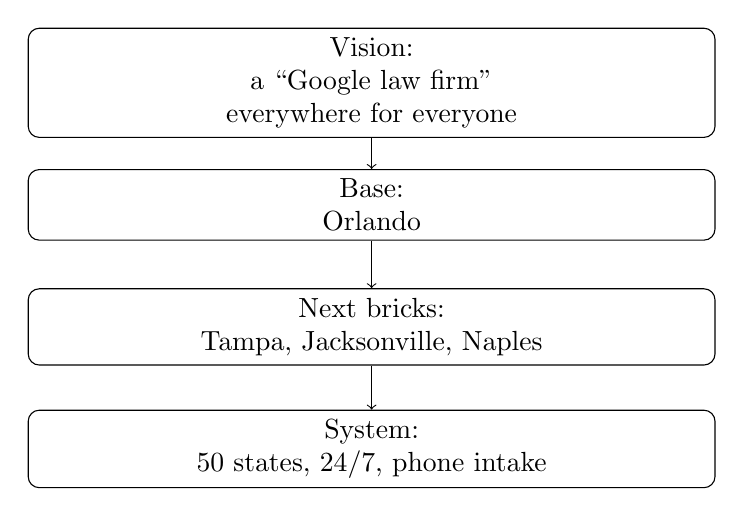
\begin{tikzpicture}[x=1cm,y=1cm]
\node[draw, text width=.70\linewidth, align=center, rounded corners] (vision) at (0,0) {Vision:\\ a ``Google law firm''\\ everywhere for everyone};
\node[draw, text width=.70\linewidth, align=center, rounded corners] (base) at (0,-1.55) {Base:\\ Orlando};
\node[draw, text width=.70\linewidth, align=center, rounded corners] (bricks) at (0,-3.10) {Next bricks:\\ Tampa, Jacksonville, Naples};
\node[draw, text width=.70\linewidth, align=center, rounded corners] (system) at (0,-4.65) {System:\\ 50 states, 24/7, phone intake};

\draw[->] (vision) -- (base);
\draw[->] (base) -- (bricks);
\draw[->] (bricks) -- (system);
\end{tikzpicture}
\caption{Transcript-grounded reconstruction of Morgan's expansion logic: large distribution vision, built through local operating increments.}
\end{figure}

The brick metaphor matters. It protects the reader from confusing aspiration with infrastructure. A national firm is not made national by announcing a national ambition. It is made national by repeating a unit that can stand up under pressure.

\section{Marketing Catches Fish; Lawyers Cook Fish}

The strongest arithmetic arrives near the end. Morgan states that the firm spends about \$400 million a year on advertising and did about \$5 billion in settlements and verdicts. The host observes that the advertising figure is less than 10 percent of the settlements-and-verdicts figure. The calculation is:

\begin{align}
A_{\mathrm{advertising}} &= \$400\mathrm{M},\\
V_{\mathrm{settlements+verdicts}} &= \$5\mathrm{B},\\
\frac{A_{\mathrm{advertising}}}{V_{\mathrm{settlements+verdicts}}}
&=
\frac{400\mathrm{M}}{5\mathrm{B}}
=
0.08
=
8\%
<
10\%.
\end{align}

This is useful arithmetic, but we have to keep it in its lane. It is not profit margin. It is not audited return on advertising. It is a transcript-backed ratio between two stated quantities.

Morgan then gives the mechanism: there are two things in his business, catching fish and cooking fish. Catching fish is client acquisition: advertising, brand, and incoming cases. Cooking fish is legal execution: lawyers who can actually get verdicts. He says the insurance industry knows who wins, names Colossus as software used by insurers, and argues that opponents know when his firm is ready to fight.

\begin{figure}
\centering
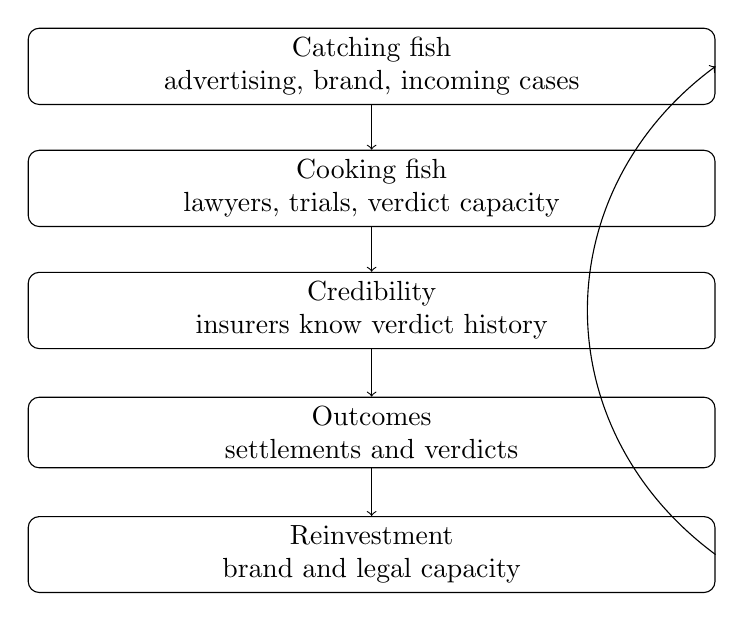
\begin{tikzpicture}[x=1cm,y=1cm]
\node[draw, text width=.70\linewidth, align=center, rounded corners] (catch) at (0,0) {Catching fish\\ advertising, brand, incoming cases};
\node[draw, text width=.70\linewidth, align=center, rounded corners] (cook) at (0,-1.55) {Cooking fish\\ lawyers, trials, verdict capacity};
\node[draw, text width=.70\linewidth, align=center, rounded corners] (cred) at (0,-3.10) {Credibility\\ insurers know verdict history};
\node[draw, text width=.70\linewidth, align=center, rounded corners] (outcome) at (0,-4.65) {Outcomes\\ settlements and verdicts};
\node[draw, text width=.70\linewidth, align=center, rounded corners] (reinvest) at (0,-6.20) {Reinvestment\\ brand and legal capacity};

\draw[->] (catch) -- (cook);
\draw[->] (cook) -- (cred);
\draw[->] (cred) -- (outcome);
\draw[->] (outcome) -- (reinvest);
\draw[->] (reinvest.east) .. controls (2.2,-4.6) and (2.2,-1.6) .. (catch.east);
\end{tikzpicture}
\caption{The operating loop implied by Morgan's catching-fish/cooking-fish metaphor. Marketing creates cases; legal capacity makes those cases valuable.}
\end{figure}

Morgan says the firm has about 200 trial dockets each week:

\begin{equation}
d_{\mathrm{trial\ dockets}}
\approx
200\ \mathrm{per\ week}.
\end{equation}

That number is the bridge between advertising and seriousness. If the firm can advertise but cannot try cases, Morgan says it is a paper tiger. If it can both attract clients and credibly fight large defendants, the advertising has something real behind it.

\begin{table}
\centering
\begin{tabular}{|p{.43\linewidth}|p{.43\linewidth}|}
\hline
Transcript-backed quantity & Role in the mechanism\\
\hline
\(\$1.5\mathrm{B}\) Forbes-attributed net worth & Opening status claim\\
\hline
\(\$2\mathrm{B}\) annual fees & Firm scale claim\\
\hline
\(\$400\mathrm{M}\) advertising & Client acquisition engine\\
\hline
\(\$5\mathrm{B}\) settlements and verdicts & Outcome scale claim\\
\hline
\(200\) weekly dockets & Trial readiness claim\\
\hline
\(50\) states, \(24/7\) & Distribution model\\
\hline
\(4\%\) to \(4.5\%\) tax-free bond yield & Wealth-preservation claim\\
\hline
\end{tabular}
\caption{Selected numerical claims from the interview. They are preserved as source-grounded business arithmetic, not independent verification.}
\end{table}

\section{Keeping Money: Greed, Black Swans, No Debt, and Giving}

The final movement shifts from making money to keeping it. Morgan says it is hard to make money and harder to keep money. His named enemy is greed: doing something one knows is wrong because the promise looks too attractive. His rule is simple enough to keep in plain language: if it is too good to be true, it is too good to be true.

The investment list is conservative and concrete. He mentions \emph{A Random Walk Down Wall Street} and \emph{Black Swan}. He says he uses index funds for equities, tax-free bonds yielding about 4 to 4.5 percent, U.S. Treasuries, and operating assets he understands: attractions, hotels, shopping centers, and apartments. Once money goes into investments, he says, he does not touch it.

We can write the allocation as a set of transcript-backed categories:

\begin{equation}
\mathcal{P}
=
\{
\mathrm{index\ funds},
\mathrm{tax\mbox{-}free\ bonds},
\mathrm{Treasuries},
\mathrm{owned\ operating\ assets}
\}.
\end{equation}

His Black Swan lesson is not presented as a technical theory. Morgan extracts one practical rule: be prepared.

\begin{equation}
\mathrm{Preparedness}
=
\mathrm{savings}
+
\mathrm{no\ debt}
+
\mathrm{readiness\ for\ discontinuity}.
\end{equation}

This is where the earlier debt equation becomes more than a boast. In Morgan's telling, leverage is fragility. He compares leveraged business people to players in musical chairs: when the music stops, the question is whether one has a chair.

The closing then returns from balance sheets to character. On branding, Morgan says to make the creative creative, but also to build trust for the long haul. People want a winner and a fighter. For a final principle, he gives the golden rule. For later advice, he names \emph{Give and Take}: people who give without expecting immediate return often receive the most over time.

The closing mechanism is therefore a trust loop:

\begin{equation}
\mathrm{Giving}
\longrightarrow
\mathrm{trust}
\longrightarrow
\mathrm{relationships}
\longrightarrow
\mathrm{opportunity}.
\end{equation}

The interview begins with the spectacle of a billionaire lawyer. It ends with a stricter claim: wealth survives through shared upside, reputation, preparedness, and the discipline not to extract from every relationship at once.

\section{Summary}

Morgan's interview gives a model of wealth built from a profession, but not from professional labor alone. The path described in the transcript combines contingency-fee upside, trusted partners, a personal mission, national distribution, heavy advertising, trial capacity, reputation, and conservative personal risk management.

The central arithmetic is the comparison between \$400 million of advertising and \$5 billion of settlements and verdicts, which gives an 8 percent ratio. The central mechanism is more important than the ratio: catching fish requires marketing, cooking fish requires lawyers, and the firm needs both. The final discipline is preservation. Morgan's rules are to avoid greed, avoid what he does not understand, prepare for the Black Swan, carry no debt, keep one's word, and give more than one tries to take.